\documentclass[12pt, a4paper]{article}
\usepackage[lmargin=3cm,rmargin=2cm,tmargin=3cm,bmargin=2cm]{geometry}
\usepackage[utf8]{inputenc}
\usepackage[T1]{fontenc}
\usepackage{titling}
\usepackage[brazil]{babel}
\usepackage{enumerate,setspace,graphicx,amsmath,tikz,amsfonts,amssymb}
\usepackage{indentfirst}
\usepackage{lmodern}
\usepackage{color}
\usepackage{hyperref}
\usepackage[alf]{abntex2cite}
\usepackage{url}
\usepackage{float}
\usepackage[skip=10pt]{caption}

% Formatação do artigo
\onehalfspacing
\setlength{\parindent}{1.25cm}
\setlength{\parskip}{0.2cm}

% Configurações do título e autores
\pretitle{\raggedright\large\bfseries}
\posttitle{\par\vspace{0.1em}}
\preauthor{\raggedright\small}
\postauthor{\par\vspace{-5em}}

% Título e autores
\title{Avaliação Comparativa de Algoritmos em Diferentes Linguagens de Programação: Impacto no Desempenho e Eficiência Computacional}
\author{Guilherme Cavenaghi (Fundação Hermínio Ometto) guilherme.cavenaghi@alunos.fho.edu.br}
\date{}

\begin{document}
\pagenumbering{gobble}

\maketitle

% Resumo alinhado à esquerda
\begin{flushleft}
\section*{Resumo}
\noindent Este trabalho apresenta uma análise comparativa de desempenho de algoritmos de classes polinomiais implementados em múltiplas linguagens de programação. O estudo busca avaliar métricas como tempo de execução, uso de memória e complexidade de implementação, considerando diferentes paradigmas de execução e modelos de tipagem. A investigação tem como objetivo identificar potenciais impactos da linguagem de programação na eficiência computacional, fornecendo subsídios para decisões fundamentadas em contextos de desenvolvimento e pesquisa. A abordagem adotada inclui experimentos controlados e repetidos para garantir confiabilidade estatística, permitindo a comparação rigorosa entre as linguagens avaliadas. Espera-se, com isso, contribuir para o entendimento do papel das linguagens de programação no desempenho de algoritmos, orientando escolhas tecnológicas em projetos computacionais de diferentes naturezas.

\vspace{0.15cm}
\noindent\textbf{Palavras-chave:} algoritmos, linguagens de programação, desempenho computacional, análise de complexidade, eficiência de execução.
\end{flushleft}


% 1. Introdução
\section{Introdução}
O desenvolvimento de software de alta qualidade e desempenho constitui um aspecto central da computação, uma vez que a eficiência computacional afeta diretamente o tempo de execução, o consumo de recursos e a escalabilidade das aplicações. Nesse contexto, a escolha da linguagem de programação emerge como uma variável determinante, influenciando a forma como algoritmos são implementados e executados, impactando, consequentemente, o desempenho geral dos sistemas. Embora a lógica algorítmica seja, em essência, independente da linguagem, fatores como modelo de execução (interpretado ou compilado), gerenciamento de memória (manual ou automático), tipagem (estática ou dinâmica) e otimizações aplicadas pelos compiladores ou interpretadores introduzem variações significativas no comportamento prático dos algoritmos, como destaca \citeonline{sebesta2016}.

Apesar da reconhecida importância desse tema, observa-se na literatura uma lacuna no que diz respeito a estudos empíricos que abordem comparativamente o impacto das linguagens de programação no desempenho de algoritmos. A maioria dos trabalhos existentes limita-se a análises conceituais ou relatos de experiências pontuais, carecendo de experimentação controlada e de dados quantitativos robustos que permitam fundamentar decisões de escolha de linguagem em cenários computacionais diversos. Tal lacuna evidencia a necessidade de investigações sistemáticas que transcendam discussões meramente subjetivas e contribuam para a consolidação do conhecimento científico na área.

A relevância desta pesquisa decorre, portanto, da necessidade de orientar desenvolvedores e pesquisadores na seleção mais adequada de linguagens de programação, considerando não apenas critérios subjetivos de preferência ou familiaridade, mas também evidências empíricas de desempenho, uso de memória e complexidade de implementação. Essa fundamentação é especialmente importante em aplicações críticas que demandam alto desempenho e confiabilidade, impactando diretamente a produtividade e a eficiência dos sistemas de software.

A motivação central deste trabalho reside na percepção de que, em um cenário de crescente diversidade de linguagens de programação e de demandas por eficiência, torna-se imperativo compreender como diferentes linguagens se comportam na implementação de algoritmos fundamentais. Tal compreensão possibilita não apenas a escolha racional de tecnologias, mas também a identificação de trade-offs relevantes entre desempenho e produtividade, contribuindo para o aprimoramento da qualidade de projetos de software em ambientes acadêmicos e industriais.

Diante desse panorama, este trabalho tem como objetivo principal realizar uma análise comparativa do desempenho de algoritmos clássicos pertencentes à classe polinomial, considerando diferentes linguagens de programação. Busca-se, assim, fornecer uma base empírica que auxilie na tomada de decisões fundamentadas acerca da escolha de linguagem, considerando o impacto de diferentes paradigmas de execução e características de implementação no desempenho computacional.

\section{Referencial Teórico}

\subsection{Teoria da Complexidade Computacional}

A teoria da complexidade computacional estuda a classificação de problemas de acordo com os recursos necessários para resolvê-los, como tempo e memória. Essa classificação é essencial para compreender as limitações práticas e teóricas na execução de algoritmos e fundamenta a análise comparativa de linguagens de programação.  

\subsubsection{Modelos de Computação}

O modelo de máquina de Turing é a base teórica para definição de complexidade, permitindo a formalização de algoritmos e problemas computacionais. Para um problema de decisão, define-se \( T(n) \) como a função de tempo que representa o número de passos que a máquina executa para resolver o problema de entrada de tamanho \( n \).

\subsubsection{Classes de Complexidade Polinomial}

Neste trabalho, o foco recai sobre as classes de complexidade polinomial, fundamentais para a análise comparativa de desempenho computacional. A Figura~\ref{fig:complexidade} ilustra as principais relações entre essas classes de complexidade. São elas:

\begin{itemize}
    \item \textbf{Classe P}: Inclui problemas solucionáveis por algoritmos determinísticos em tempo polinomial. Formalmente:
    \[
    T(n) = O(n^k)
    \]
    para alguma constante \( k \). Essa classe representa problemas considerados tratáveis na prática, como o MergeSort (\( O(n \log n) \)) \citeonline{knuth1998}.

    \item \textbf{Classe NP}: Compreende problemas cujas soluções podem ser verificadas em tempo polinomial, mesmo que não exista algoritmo determinístico conhecido para resolvê-los em tempo polinomial. Para todo \( L \in \text{NP} \), existe um verificador determinístico \( V(x,y) \):
    \[
    V(x, y) = \text{Sim ou Não}
    \]
    com:
    \[
    T_V(|x| + |y|) = O((|x| + |y|)^k)
    \]
    Exemplo: Satisfatibilidade Booleana (SAT) \citeonline{garey1979}.

    \item \textbf{Classe NP-completo}: Engloba problemas para os quais qualquer problema em NP pode ser reduzido a eles em tempo polinomial. Para \( A \) ser NP-completo:
    \[
    A \in \text{NP} \quad \text{e} \quad \forall B \in \text{NP}, \quad B \leq_P A
    \]
    onde \( B \leq_P A \) indica uma redução polinomial. Exemplo: Problema da Mochila (Knapsack) \citeonline{garey1979}.

    \item \textbf{Classe NP-difícil}: Abrange problemas que são no mínimo tão difíceis quanto qualquer problema de NP, podendo ser ou não verificáveis em tempo polinomial. Para \( A \) ser NP-difícil:
    \[
    \forall B \in \text{NP}, \quad B \leq_P A
    \]
    Muitos desses problemas são indecidíveis, como o Problema da Parada (Halting Problem), definido por:
    \[
    \text{HALT}(P,x) = 
    \begin{cases}
    \text{Sim}, & \text{se } P(x) \text{ termina} \\
    \text{Não}, & \text{caso contrário}
    \end{cases}
    \]
    O Teorema de Turing demonstra que HALT é indecidível, não existindo algoritmo que resolva o problema para todas as entradas \citeonline{sipser2012}.
\end{itemize}

\begin{figure}[H]
    \centering
    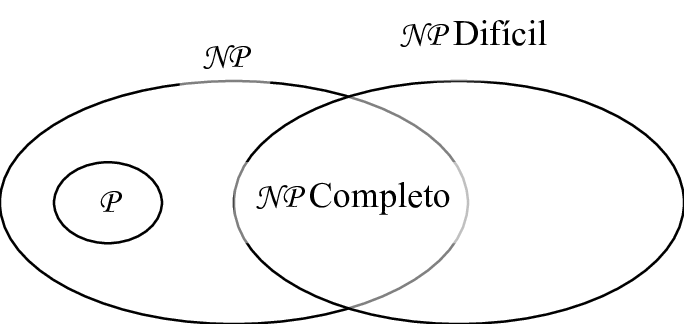
\includegraphics[width=0.5\textwidth]{img/relacaoDeConjuntos.png}
    \caption{Diagrama das classes de complexidade P, NP, NP-completo e NP-difícil.}
    \label{fig:complexidade}
\end{figure}
\subsection{Algoritmos Fundamentais}

Os algoritmos utilizados para análise de desempenho são representativos das classes polinomiais e foram escolhidos considerando sua relevância teórica e aplicabilidade prática.

\subsubsection{Ordenação}

O algoritmo MergeSort é representativo da classe P e é amplamente utilizado devido à sua complexidade \( O(n \log n) \). Sua estrutura de divisão e conquista permite uma ordenação eficiente, servindo como benchmark para linguagens de programação compiladas e interpretadas.

\subsubsection{Problemas de Otimização e Satisfatibilidade}

Problemas como o Knapsack (NP-completo) e o SAT (NP) são utilizados para avaliar a capacidade das linguagens em lidar com desafios de verificação e busca combinatória. Embora ambos sejam polinomiais em suas versões restritas neste estudo, a implementação de suas versões básicas permite comparar overheads entre linguagens.

\subsubsection{Problemas Indecidíveis}

A análise do Problema da Parada, apesar de ser indecidível em geral, é abordada de forma restrita neste trabalho (por exemplo, simulando programas com entradas controladas), possibilitando a avaliação de tempo de execução e uso de memória em linguagens diversas.

\subsection{Linguagens de Programação}

A linguagem de programação exerce impacto significativo na implementação de algoritmos, influenciando tempo de execução, uso de memória e complexidade de desenvolvimento.

\subsubsection{Critérios de Seleção}

As linguagens foram escolhidas com base em:

\begin{itemize}
    \item \textbf{Popularidade}: Métricas como o TIOBE Index \citeonline{tiobe}, GitHub Octoverse \citeonline{octoverse} e Stack Overflow Developer Survey \citeonline{stackoverflow}.
    \item \textbf{Diversidade de paradigmas}: Compiladas (C, C++, Rust), interpretadas (Python, JavaScript) e híbridas (Java, C\#, Go, Kotlin, TypeScript).
    \item \textbf{Aplicabilidade acadêmica e industrial}: Referências como Sebesta \citeonline{sebesta2016} evidenciam o uso prático e teórico das linguagens.
\end{itemize}

\subsubsection{Paradigmas e Modelos de Execução}

A diversidade de linguagens reflete diferenças como:

\begin{itemize}
    \item \textbf{Modelo de execução}: Compilado (execução direta) ou interpretado (via máquina virtual ou interpretador).
    \item \textbf{Tipagem}: Estática (C, Java) ou dinâmica (Python, JavaScript).
    \item \textbf{Gerenciamento de memória}: Manual (C, C++) ou automático (Java, Python).
\end{itemize}

Essas características influenciam diretamente o desempenho e a escalabilidade dos algoritmos, justificando a escolha das linguagens para os experimentos.


% 3. Materiais e Métodos
\section{Materiais e Métodos}

\subsection{Ambiente Experimental}

Os experimentos serão realizados em ambiente controlado, a fim de reduzir variações externas que possam interferir nas medições de desempenho. A configuração de hardware e software utilizada é a seguinte:

\begin{itemize}
    \item \textbf{Processador}: 11th Gen Intel(R) Core(TM) i7-1165G7 @ 2.80 GHz, com suporte a múltiplos threads, adequado para executar algoritmos em diferentes linguagens com boa capacidade computacional.
    \item \textbf{Memória RAM}: 16 GB DDR4 (2667 MHz), garantindo que a execução dos experimentos ocorra sem restrições de memória para os tamanhos de entrada definidos.
    \item \textbf{Placa de Vídeo}: Intel(R) Iris(R) Xe Graphics com 128 MB de memória dedicada, suficiente para suportar ambientes gráficos e alguns experimentos que exigem renderização leve.
    \item \textbf{Sistema Operacional}: Ubuntu 22.04 LTS, escolhido por sua estabilidade, suporte a múltiplas linguagens de programação e ferramentas robustas de monitoramento de desempenho.
\end{itemize}

Essa infraestrutura assegura uniformidade na execução dos algoritmos, minimizando influências externas como processos em segundo plano ou gerenciadores de energia.

\subsection{Métricas}

Para cada combinação de algoritmo e linguagem de programação, serão avaliadas as seguintes métricas:

\begin{itemize}
    \item \textbf{Tempo de Execução (Wall Clock Time)}: Medido como a média de 30 execuções consecutivas, utilizando o tempo de relógio total decorrido (e não apenas tempo de CPU). Essa métrica captura o tempo real de execução percebido pelo usuário, incluindo overheads do interpretador ou da máquina virtual.
    \item \textbf{Uso de Memória (RSS)}: Obtido a partir do utilitário \texttt{/usr/bin/time}, considerando o pico de uso de memória residente (Resident Set Size) durante a execução. Essa métrica reflete a demanda de memória real, incluindo buffers e alocações dinâmicas.
    \item \textbf{Complexidade de Implementação}: Avaliada por meio de Linhas de Código Fonte (SLOC) e Complexidade Ciclomática (McCabe). O SLOC fornece uma medida quantitativa da extensão do código-fonte, enquanto a Complexidade Ciclomática indica a quantidade de caminhos lógicos distintos, fornecendo uma proxy para a manutenção e legibilidade do algoritmo.
\end{itemize}

A escolha dessas métricas justifica-se pela necessidade de compreender não apenas o desempenho absoluto (tempo e memória), mas também o esforço de implementação associado a cada linguagem de programação.

\subsection{Conjuntos de Dados}

Serão utilizados conjuntos de dados sintéticos escaláveis, projetados para garantir reprodutibilidade e permitir análises comparativas em diferentes ordens de grandeza. Os tamanhos de entrada foram definidos com base na complexidade assintótica dos algoritmos implementados, respeitando a classe polinomial analisada no referencial teórico:

\begin{itemize}
    \item \textbf{Pequeno}: \( n = 10^3 \), representando cenários de entrada modestos, nos quais o overhead da linguagem pode ter impacto relevante.
    \item \textbf{Médio}: \( n = 10^4 \), para avaliar o comportamento intermediário e transições de eficiência entre linguagens compiladas e interpretadas.
    \item \textbf{Grande}: \( n = 10^5 \), simulando cargas intensivas de dados e testando a escalabilidade prática dos algoritmos implementados.
\end{itemize}

Cada conjunto de dados será gerado aleatoriamente, assegurando diversidade de instâncias e evitando vieses que possam privilegiar alguma linguagem específica.

\subsection{Procedimentos Experimentais}

Para cada linguagem de programação e algoritmo, o procedimento experimental será conduzido conforme os seguintes passos:

\begin{enumerate}
    \item Implementação dos algoritmos em todas as linguagens, utilizando boas práticas de codificação e bibliotecas padrão sempre que possível, para evitar otimizações artificiais.
    \item Compilação (para linguagens compiladas) ou configuração do interpretador (para linguagens interpretadas) com parâmetros padrão, garantindo uniformidade na execução.
    \item Execução dos testes de forma repetida (30 vezes) para cada tamanho de entrada, coletando as métricas definidas anteriormente.
    \item Armazenamento e análise estatística dos resultados, utilizando medidas de tendência central (média e mediana) e variabilidade (desvio padrão).
\end{enumerate}

% 4. Resultados Esperados
\section{Resultados Esperados}

\subsection{Desempenho por Classe de Algoritmo}

Com base na literatura técnica \citeonline{cormen2022,sebesta2016} e na fundamentação teórica apresentada, antecipa-se que algoritmos classificados na Classe P, como o MergeSort, apresentem desempenho superior quando implementados em linguagens compiladas (por exemplo, C e Rust) em relação a linguagens interpretadas (como Python e JavaScript). Isso se deve principalmente à compilação nativa, que elimina a sobrecarga associada a interpretadores e máquinas virtuais, conforme discutido por \citeonline{sebesta2016}. Para entradas de tamanho médio e grande (\( n \geq 10^4 \)), estima-se que linguagens compiladas possam ser de três a cinco vezes mais rápidas do que linguagens interpretadas, graças a otimizações de tempo de compilação e execução mais eficiente. Além disso, espera-se que linguagens como C++ se beneficiem de técnicas de otimização estática, proporcionando resultados consistentes em termos de tempo de execução, especialmente para algoritmos como o Knapsack, cuja análise de complexidade e estrutura algorítmica são amplamente detalhadas por \citeonline{cormen2022}.

Para problemas da Classe NP, como SAT, espera-se que linguagens com gerenciamento automático de memória e otimizações de execução just-in-time (JIT), como Java e Go, apresentem bom equilíbrio entre tempo de execução e consumo de memória. Em problemas NP-completos como Knapsack, o uso de recursos (tempo e memória) tende a crescer exponencialmente com o tamanho da entrada. Ainda assim, linguagens como C++ devem apresentar vantagem devido à eficiência de compilação e ao controle de memória manual, possibilitando otimizações específicas para entradas grandes.

Em problemas NP-difíceis e indecidíveis como o Problema da Parada (restrito), prevê-se que o impacto da linguagem seja menos significativo em termos absolutos, uma vez que a complexidade teórica domina o crescimento do tempo de execução. Entretanto, linguagens como Rust e C ainda devem ter vantagens por apresentarem menor overhead de execução e gerenciamento de recursos mais direto.

\subsection{Consumo de Memória}

Em relação ao uso de memória, espera-se que linguagens com coleta de lixo (garbage collection), como Java e Go, apresentem overhead de aproximadamente 2x em comparação a linguagens como C e Rust. Esse overhead decorre da gestão automática de memória e da necessidade de estruturas de dados intermediárias para o gerenciamento de objetos.

Linguagens como Rust e C, por possuírem gerenciamento de memória manual (ou ownership estático, no caso de Rust), devem manter uso de memória mais constante, independentemente do tamanho da entrada. Isso é particularmente importante em experimentos com entradas grandes (\( n \geq 10^5 \)), onde o controle preciso do uso de memória pode evitar page faults e swapping, garantindo resultados mais consistentes.

Para linguagens interpretadas como Python e JavaScript, antecipa-se crescimento não linear no uso de memória para problemas NP e NP-completos, devido ao uso intensivo de estruturas de dados dinâmicas (listas, dicionários) e ao overhead da máquina virtual ou interpretador. Esse crescimento pode impactar a escalabilidade dos algoritmos, especialmente para instâncias de problemas combinatórios.

\subsection{Complexidade de Implementação}

Além do tempo e da memória, espera-se que a complexidade de implementação (medida em SLOC e Complexidade Ciclomática) varie significativamente entre as linguagens. Linguagens como Python e JavaScript devem apresentar menor SLOC devido à sintaxe concisa e à tipagem dinâmica, facilitando a prototipagem. Em contrapartida, linguagens como C e C++ tendem a exigir maior verbosidade, aumentando o SLOC e potencialmente a complexidade ciclomatica, em virtude da necessidade de gerenciamento manual de recursos e da ausência de abstrações de alto nível.

Linguagens híbridas (Java, C\#, Go, Kotlin, TypeScript) devem apresentar valores intermediários de complexidade de implementação, beneficiando-se de recursos como garbage collection e tipagem estática, ao mesmo tempo em que mantêm legibilidade e concisão moderadas.

\subsection{Relação entre Paradigmas e Desempenho}

Prevê-se que as linguagens compiladas apresentem melhor desempenho geral em tarefas CPU-bound (como ordenação e busca), enquanto linguagens interpretadas podem apresentar overheads significativos em algoritmos que realizam muitas iterações ou alocações de memória. Linguagens híbridas, por sua vez, devem equilibrar desempenho e facilidade de implementação, beneficiando-se de JIT e otimizações em tempo de execução.

\subsection{Síntese dos Resultados Esperados}

De forma consolidada, espera-se:

\begin{itemize}
    \item \textbf{Desempenho superior} para linguagens compiladas (C, Rust) em problemas de Classe P e NP-completo;
    \item \textbf{Equilíbrio entre tempo e memória} para linguagens híbridas (Java, Go) em problemas de Classe NP;
    \item \textbf{Overhead significativo de memória} em linguagens com garbage collection (Java, Go);
    \item \textbf{Crescimento não linear de memória} em linguagens interpretadas (Python, JavaScript) para problemas combinatórios;
    \item \textbf{Maior concisão de código} em linguagens dinâmicas, contrastando com maior SLOC e complexidade ciclomatica em linguagens como C e C++.
\end{itemize}

% REFERÊNCIAS
\bibliographystyle{abntex2-alf}
\bibliography{Bibliografia}

\end{document}
